\documentclass{beamer}
\usepackage{graphicx}
\usepackage{booktabs}
\usepackage{hyperref}
\usetheme{Madrid}

% Add your name as subtitle for title slide
\subtitle{Presented by Rousomanis Georgios (10703)}

% Footer customization: your name on bottom left of each slide
\setbeamertemplate{footline}{
  \leavevmode%
  \hbox{%
    \begin{beamercolorbox}[wd=.5\paperwidth,ht=2.5ex,dp=1ex,left]{author in head/foot}%
      \hspace{1em}Rousomanis Georgios
    \end{beamercolorbox}%
    \begin{beamercolorbox}[wd=.5\paperwidth,ht=2.5ex,dp=1ex,right]{date in head/foot}%
      \insertframenumber{} / \inserttotalframenumber\hspace{1em}
    \end{beamercolorbox}%
  }%
  \vskip0pt%
}

\title[CHROMOSOME RTE]{CHROMOSOME: A Plug \& Play-Capable Run-Time Environment for Embedded Real-Time Systems}
\author{Buckl et al., 2014}
\institute{fortiss GmbH \& Technische Universität München}
\date{May 2025}

\begin{document}

% TITLE
\begin{frame}
  \titlepage
\end{frame}

% SLIDE 1
\begin{frame}{Motivation: Why Adaptive Embedded Systems?}
  \begin{itemize}
    \item Traditional embedded systems rely on static configuration -- no updates post-deployment.
    \item New-generation systems must support:
    \begin{itemize}
      \item Dynamic integration of new functionality (e.g., OTA updates).
      \item Adaptation to topology changes (e.g., nodes joining or leaving a network).
    \end{itemize}
    \item Existing run-time systems (e.g., RTOS):
    \begin{itemize}
        \item \textit{Pro}: guaranteed satisfaction of requirements (e.g., real-time behavior, safety)
        \item \textit{Con}: rely on a static configuration to satisfy requirements
    \end{itemize}
    \item Web-service-style middleware (e.g., cloud, enterprise systems)
    \begin{itemize}
        \item \textit{Pro}: satisfy adaptability requirements -- very flexible
        \item \textit{Con}: do not guarantee fulfillment of resource constraints
    \end{itemize}
    \item Challenge: Combine plug \& play capabilities with hard real-time guarantees.
  \end{itemize}
\end{frame}

% SLIDE 2
\begin{frame}{CHROMOSOME (XME): What Is It?}
  \begin{itemize}
    \item A modular run-time environment designed for embedded real-time systems.
    \item Built to support plug \& play at both software and network levels.
    \item Cross-platform and open-source -- usable across industrial and automotive domains.
    \item Resource-aware: Uses lookup tables to ensure that added components fit system limits.
    \item Components are dynamically loaded only if sufficient memory, CPU time, and bandwidth exist.
    \item Compatible with both time-triggered and event-driven execution models.
  \end{itemize}
\end{frame}

% SLIDE 3
\begin{frame}{Core Concepts of XME}
  \begin{itemize}
    \item \textbf{Requirements-centric design}: Application developers specify constraints like WCET, latency, safety level.
    \item \textbf{Data-centric communication}: No hard-coded connections; communication defined by topic types and attributes.
    \item \textbf{Plug \& play orchestration}: New nodes/components can register and integrate safely at run-time.
    \item \textbf{Shadow configuration}: Ensures system consistency during reconfiguration — existing tasks are not interrupted.
    \item \textbf{Topic dictionaries}: Promote interoperability across independently developed modules.
    \item \textbf{Modularity}: Different runtime components (e.g., schedulers) can be selected per platform.
  \end{itemize}
\end{frame}

% SLIDE 4
\begin{frame}{Communication via Topics and Dictionaries}
  \begin{itemize}
    \item XME replaces traditional service calls with publish/subscribe over semantic “topics.”
    \item Each topic includes:
    \begin{itemize}
      \item Data type (e.g., sensor\_reading, vehicle\_position).
      \item Qualifiers: min/max range, units, criticality level, precision.
    \end{itemize}
    \item Topic matching ensures syntactic and semantic compatibility between components.
    \item Enables components developed independently to interoperate safely.
  \end{itemize}
\end{frame}

% SLIDE 5
\begin{frame}{XME Architecture Overview}
  \begin{itemize}
    \item The XME ecosystem is a federation of runtime nodes.
    \item Each node includes core services: Execution Manager, Broker, Data Handler, PAL.
    \item Nodes communicate via directed, type-safe publish-subscribe channels.
    \item The architecture separates application logic from low-level hardware using PAL.
    \item Reconfiguration is handled by plug-phase components: Login and Plug \& Play Managers.
    \item Adaptivity features are only enabled if the node includes plug-phase services.
  \end{itemize}
\end{frame}

% SLIDE 6
\begin{frame}{XME Architecture Overview}
  \begin{figure}
      \centering
      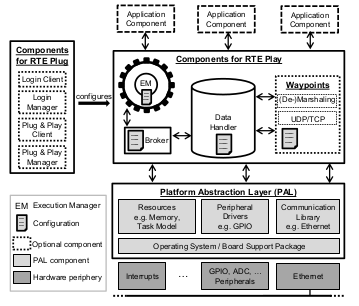
\includegraphics[width=0.6\linewidth]{XME_architecture.png}
  \end{figure}
\end{frame}

% SLIDE 7
\begin{frame}{Play-Phase Components}
  \begin{itemize}
    \item \textbf{Execution Manager (EM)}:
    \begin{itemize}
      \item Invokes application components according to their priority and WCET.
      \item Monitors for timing violations; reports if a task exceeds limits.
    \end{itemize}
    \item \textbf{Broker}:
    \begin{itemize}
      \item Watches data subscriptions and enables components only when inputs are ready.
    \end{itemize}
    \item \textbf{Data Handler}:
    \begin{itemize}
      \item Provides a consistent data interface to components.
      \item Ensures safe, bounded-latency access to shared data.
    \end{itemize}
    \item These ensure deterministic behavior during the “play” (runtime) phase.
  \end{itemize}
\end{frame}

% SLIDE 8
\begin{frame}{Waypoints and Platform Abstraction Layer (PAL)}
  \textbf{Waypoints:}
  \begin{itemize}
    \item Lightweight modules for data transformation and verification.
    \item Can include marshaling (endianness), redundancy, CRCs, encryption, etc.
    \item Configured dynamically per data route based on system requirements.
  \end{itemize}
  \textbf{Platform Abstraction Layer (PAL):}
  \begin{itemize}
    \item Provides uniform access to hardware (GPIO, timers, interrupts).
    \item Makes applications portable across OSes like PikeOS, Linux, or even bare metal.
  \end{itemize}
\end{frame}

% SLIDE 9
\begin{frame}{Plug-Phase: Dynamic Integration in XME}
  \begin{itemize}
    \item \textbf{Login Phase:}
    \begin{itemize}
      \item New node’s \textit{Login Client} contacts a central \textit{Login Manager}.
      \item Enables access to XME services.
    \end{itemize}

    \item \textbf{Component Discovery:}
    \begin{itemize}
      \item \textit{Plug \& Play Client} sends \textit{manifests} to the \textit{Plug \& Play Manager}.
      \item Describes topics, resource needs, and constraints.
    \end{itemize}

    \item \textbf{Validation:}
    \begin{itemize}
      \item \textit{Logical Route Manager} computes routes.
      \item Configurators check network and node resource availability.
    \end{itemize}

    \item \textbf{Decision:}
    \begin{itemize}
      \item If checks pass: update lookup tables and apply new config.
      \item Else: reject change to maintain safety and real-time guarantees.
    \end{itemize}
  \end{itemize}
\end{frame}

% SLIDE 10
\begin{frame}{CHROMOSOME Modeling Tool (XMT)}
  \textbf{Purpose:} Support the design, validation, and configuration of distributed embedded systems.

  \vspace{0.7em}
  \begin{itemize}
    \item \textbf{Model-driven design tool}, built on Eclipse.
    \item Defines an iterative workflow:
    \begin{itemize}
      \item Specification → Implementation → Evolution
    \end{itemize}
    \item Allows developers to:
    \begin{itemize}
      \item Declare requirements (timing, safety, communication patterns).
      \item Model the XME ecosystem structure and topic dictionaries.
      \item Validate the system early to catch design issues.
      \item Auto-generate RTE configurations (adaptive or static).
    \end{itemize}
    \item \textbf{Static mode:} Generates an offline configuration with zero run-time overhead.
  \end{itemize}
\end{frame}

% SLIDE 11
\begin{frame}{Use Case 1: RACE (Automotive)}
  \begin{itemize}
    \item Objective: enable adaptive automotive architecture with hard real-time support.
    \item Deployed using PikeOS partitions -- each app runs in a secure container.
    \item XME runs in a master partition; manages partition communication and coordination.
    \item Real-time scheduling configured based on WCET data and component criticality.
    \item Allows runtime replacement of software modules without rebooting the ECU.
  \end{itemize}
\end{frame}

% SLIDE 12
\begin{frame}{Use Case 2: AutoPnP (Industrial Automation)}
  \begin{itemize}
    \item Targeted for factories needing reconfiguration without halting production.
    \item Hardware modules are detected at runtime; software activated accordingly.
    \item Event-triggered model handles inputs like sensor events or operator changes.
    \item Uses ROS for interoperability; XME adds plug \& play and timing control.
    \item Demonstrates flexibility in industrial robotics and assembly systems.
  \end{itemize}
\end{frame}

% SLIDE 13
\begin{frame}{Comparison with Other Frameworks}
  \begin{tabular}{l|l|l}
    \textbf{System} & \textbf{Real-Time Support} & \textbf{Adaptivity} \\
    \hline
    ROS & No & High \\
    DDS & Partial (QoS-based) & Medium \\
    FRESCOR & Contract-based & High \\
    \textbf{CHROMOSOME} & \textbf{WCET + Static Sched.} & \textbf{High + Modular}
  \end{tabular}
  \vspace{1em}
  \smallskip
  XME uniquely blends static real-time safety with dynamic reconfigurability.
\end{frame}

% SLIDE 14
\begin{frame}{Future Directions}
  \begin{itemize}
    \item Full end-to-end timing analysis across multi-node ecosystems.
    \item Binary deployment of application components, not just nodes.
    \item Security-aware middleware: role- and topic-based access control.
    \item Health monitoring and self-healing orchestration.
  \end{itemize}
\end{frame}

% SLIDE 15
\begin{frame}{Conclusion}
  \begin{itemize}
    \item XME enables real-time embedded systems to adapt safely and modularly.
    \item Combines model-driven design, static analysis, and runtime orchestration.
    \item Plug \& play becomes practical for cyber-physical systems (CPS).
    \item Publicly available -- suitable for research and industrial applications.
  \end{itemize}
\end{frame}

% SLIDE 16
\begin{frame}{Thank You!}
  \centering
  \Huge Questions?
\end{frame}

\end{document}

